\documentclass{article}

\usepackage{hyperref}
\usepackage{graphicx}
\usepackage[style=authoryear,backend=biber]{biblatex}
\usepackage[margin=1in]{geometry}
\usepackage[divipsnames]{xcolor}
\usepackage{float}
\usepackage{minted}
\usepackage{algorithm}
\usepackage{algpseudocode}


\makeatletter
\renewcommand{\ALG@name}{Pseudocode}

\bibliography{ref}

\setlength\parindent{0pt}
\setlength\parskip{0.5em}

\hypersetup{
	colorlinks = true,
	urlcolor   = blue,
	linkcolor  = blue,
	citecolor  = darkgray
}

\title{2D Procedural Map Generation \\ \large With Pascal \& SwinGame}
\author{Jacob Milligan \\ \small Student ID - 100660682}
\date{}

\begin{document}

\maketitle
	
	
\section{Procedural Generation}

\subsection{Procedural over Manual}


Very broadly speaking, in game development there are two primary ways to generate content for a project. The most common and controllable way is to make each part by hand - in our case we'll be referring to a 2D tile map as our content.
		
For small maps this isn't a problem; it's very straight-forward to declare each tile as an element of a statically-sized 2D array (we'll go into how this is done later) and just draw those tiles 	to the screen, perhaps also drawing different sprites on top of each tile for NPC's or the player. But what happens as our map grows in size? As it goes from a 32 x 32 map to a 256 x 256 sized map, or even larger? Even if we've created a system for writing our maps out as text files to be read in, already saving lots of time, this can very quickly become time-consuming. This is a valid way of generating content, in fact the developers on CD Projekt Red's The Witcher 3: Wild Hunt did just that \parencite{witcher}, a pretty amazing feat. However, we don't have the resources or manpower of CD Projekt Red, so what's the solution?
		
\paragraph{Procedural Generation algorithms are the solution}\mbox{}
		
Games such as Minecraft, Dwarf Fortress, and the upcoming No Mans Sky all make use of procedural generation to generate enormous, beautiful, but seemingly random worlds. We say \emph{seemingly} random because, aside from computers only being able to generate \emph{pseudo}-random numbers, these algorithms are designed so that, with the same starting point, it will produce the same result.
		
\paragraph{"So then where do we start?"}
		
Good question. Many games, such as in indie title Dwarf Corp. \parencite{dwarfcorp}, begin by simulating tectonic plate activity, erosion, and river formation to carve out their terrain -  in a similar process to how terrain forms in the real world \parencite[pp. 46]{huggett}. However, we're going to go a different route and start by generating a realistic height map, a 2D array of elements that hold a generated elevation value, that we'll use to base the rest of our map off. We will use this starting point to procedurally generate a map that can be navigated by the player. Along the way, we will make heavy use of the SwinGame API to handle all graphics-related functionality and briefly touch on other concepts such as basic collision detection, all of which we will code using Pascal.
	
	
\subsection{Diamonds \& Squares}


To generate a heightmap, it would be possible to design an algorithm from scratch, however that would take a long time and the result probably wouldn't be very effective, so we're going to borrow a very well-known and academically sound one called \textbf{Random Midpoint Displacement} \parencite{fournier}, also known as \textbf{the Diamond-Square Algorithm}. At its core, the purpose of this algorithm is to generate pseudo-random noise in a desirable pattern, i.e.~one that resembles a realistic spread of terrain height values. Each point of noise is stored in a data structure (in our case, a 2D array) and holds a single value - a number representing its elevation. The result is something like this:
	
\begin{figure}[H]
	\centering
	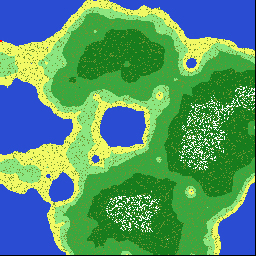
\includegraphics{map.jpg}
	\renewcommand{\figurename}{Example}
	\caption{A map generated using Diamond-Square}
\end{figure}

\paragraph{The basic concept behind Diamond-Square can be summed up like so:}
	
\begin{itemize}

	\item
		Take an empty grid which must be of size \(2^{n}+1\) in order to work. Then assign the corners a \emph{seed} value, a number that all other calculations are based off. This means that with the same seed, we should get the exact same result.
	\item
		\textbf{The Sqaure Step} - Take the grids four corners, average their total, find their mid point and assign that point the average plus a random value.
	\item
		\textbf{The Diamond Step} - Given the previous step, we now have a diamond shape surrounding a new mid point. Take the average of all points in the diamond and assign the new midpoint that value plus a random amount.
	\item
		Use a \mintinline{Pascal}{nextStep} variable to determine the next point to calculate. 
	\item
		Iterate until \mintinline{Pascal}{nextStep} is smaller than zero.
		
\end{itemize}
	
This process can be best visualized using graphs, seen in the example pictured below.
	
\begin{figure}[H]
	\centering
	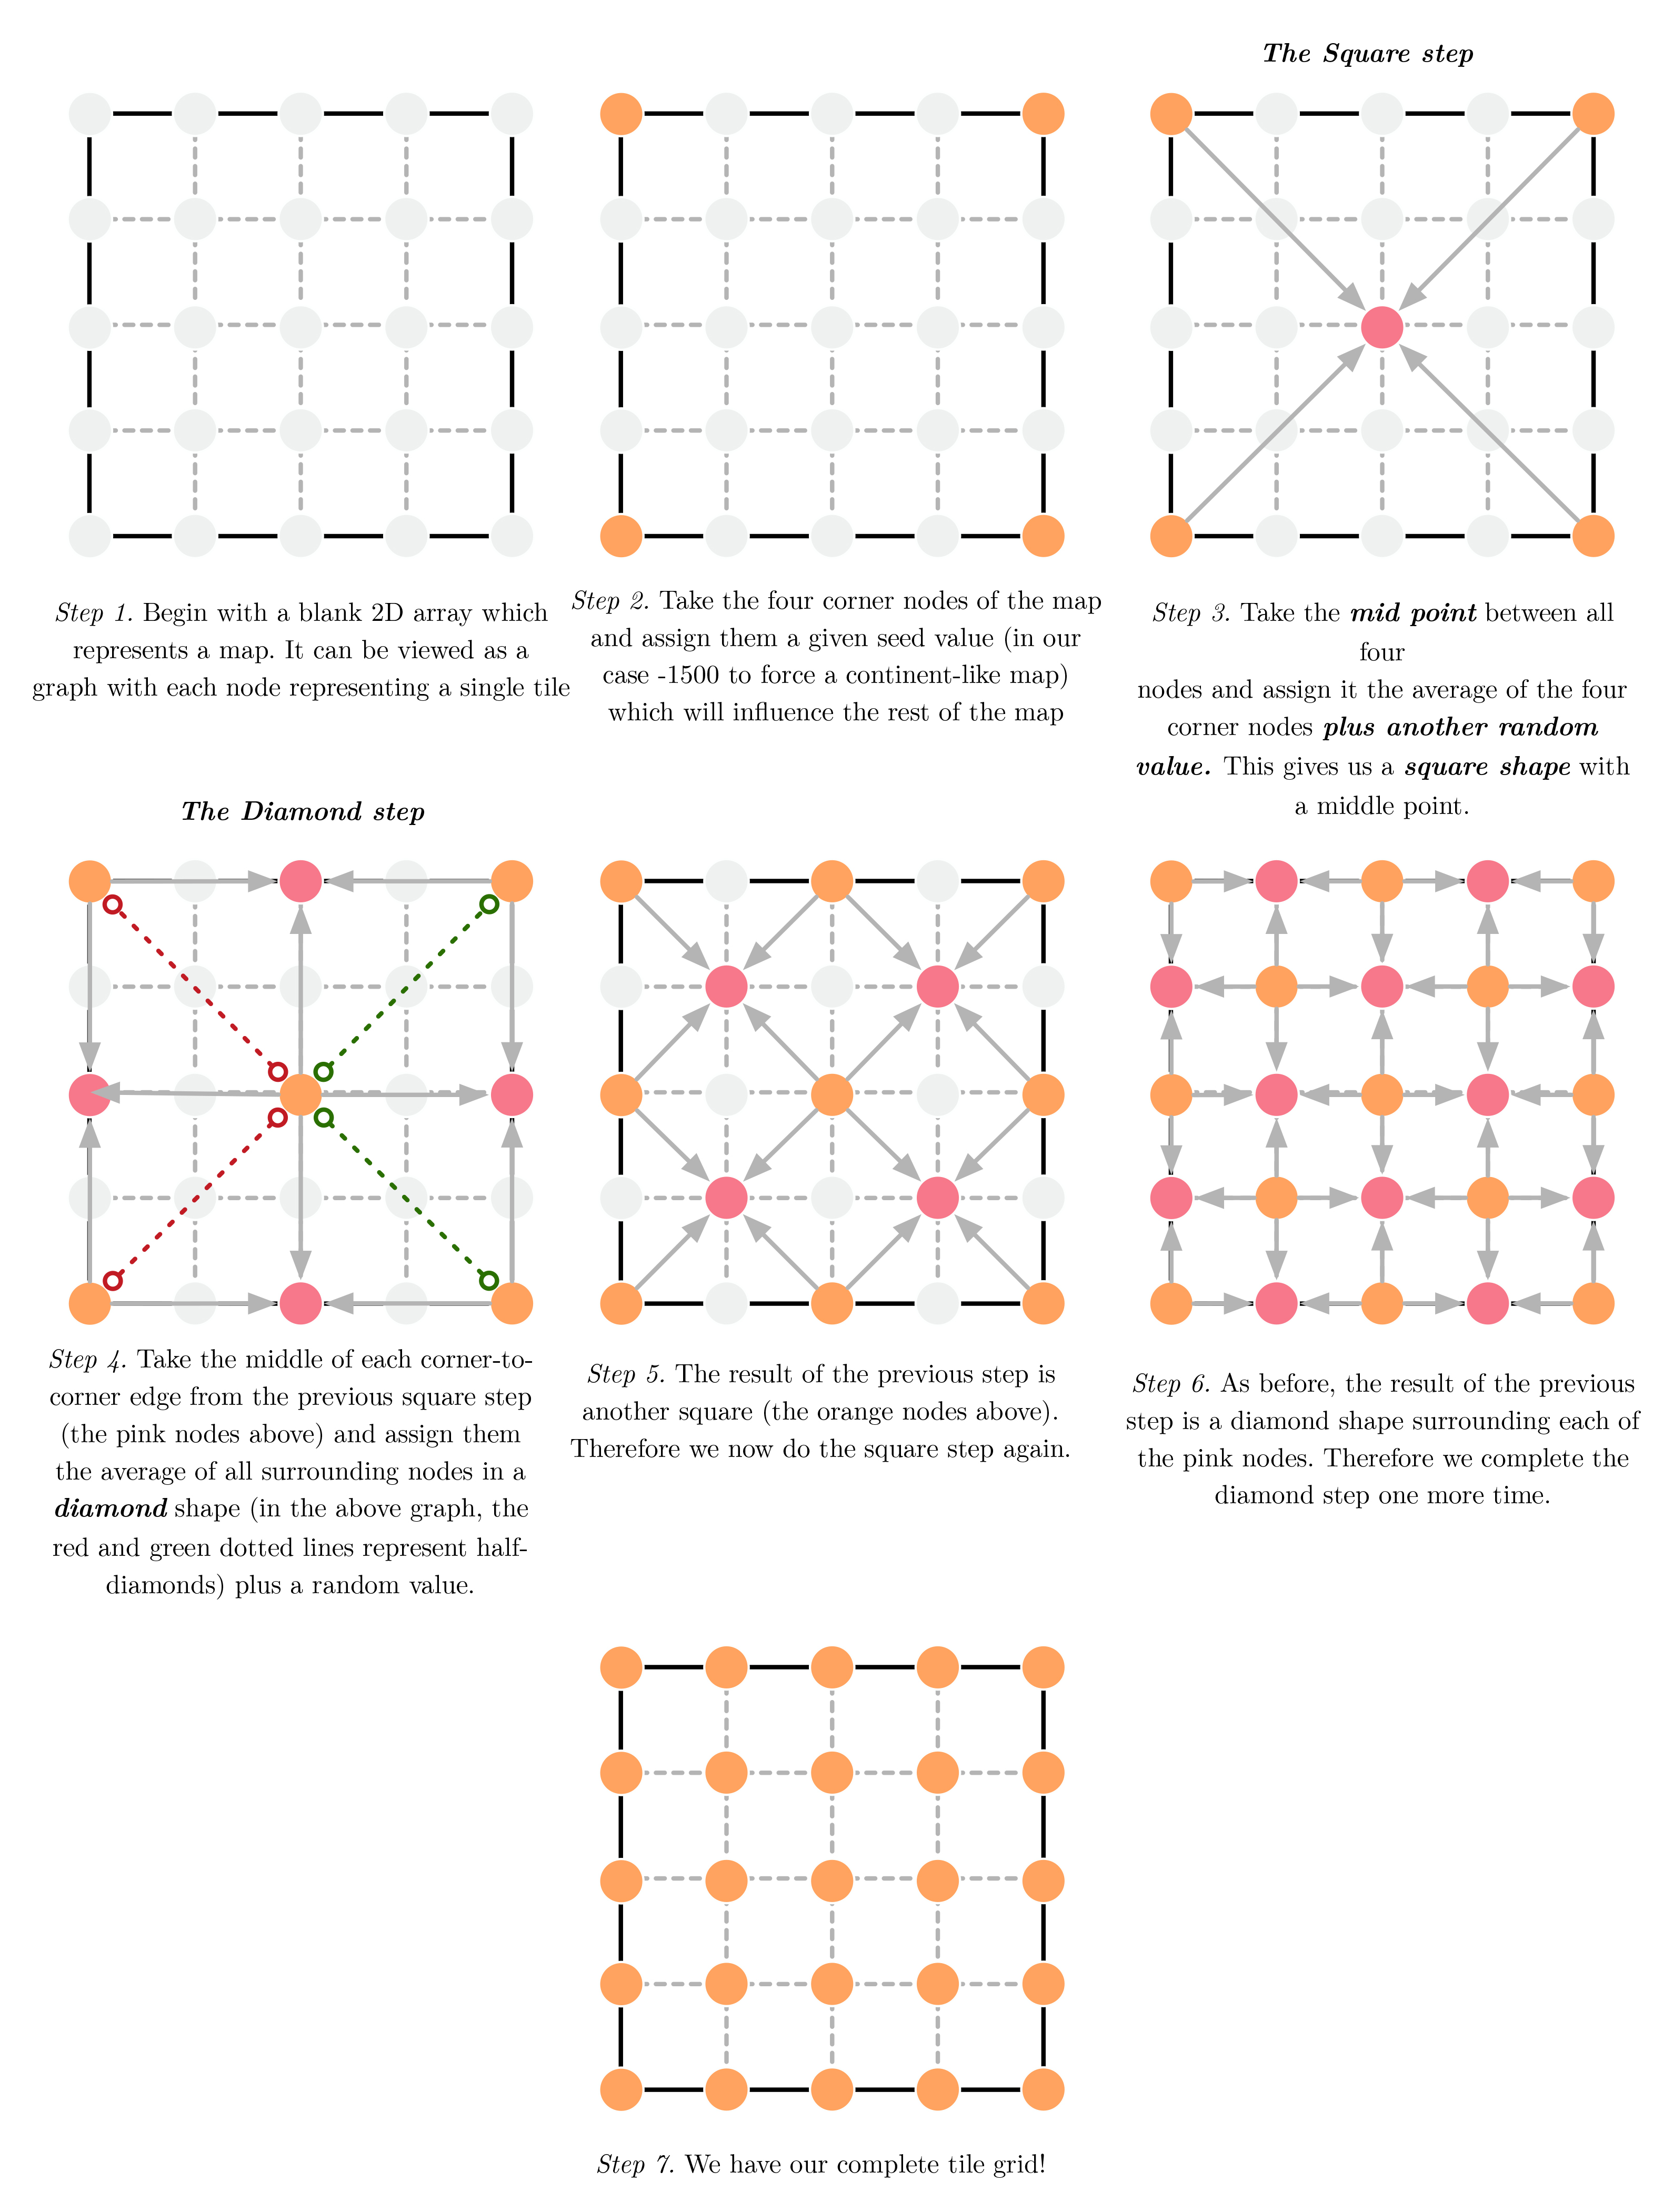
\includegraphics[width=0.9\linewidth,trim=4 4 4 4,clip]{diamondsquare.jpg}
	\renewcommand{\figurename}{Example}
	\caption{Summary of the Diamond-Square algorithm}
\end{figure}
	
\paragraph{Using this algorithm, we now have the ability to generate a starting point.}
However, before starting on an implementation, as with all software development, it's a good idea to define the requirements for our program - what functions, procedures, data structures, and features do we want to include?
	
\begin{itemize}

\item
	First, we will define the data structures that will be required by our program. We're going to first need a \mintinline{pascal}{Tile record} to hold data related to each tile in the map such as if it's collidable, the bitmap that should be drawn for it, it's type, and elevation. We'll also need a \mintinline{pascal}{MapData record} to contain our tile grid, the players sprite and location data, and its size.
\item
	Very importantly, we'll also need our terrain generation procedures - \mintinline{pascal}{DiamondSquare()} \& \mintinline{pascal}{GenerateTerrain()}. \mintinline{pascal}{DiamondSquare()} will be responsible for creating a new heightmap for a passed-in \mintinline{pascal}{MapData()} record, whereas \mintinline{pascal}{GenerateTerrain()} will be responsible for deciding how each tile should be rendered based off the heightmap, alongside generating trees on the passed-in \mintinline{pascal}{MapData()} record.
\item
	Now that our terrain generation functions and structures are defined, we'll also need a \mintinline{pascal}{CreateMap()} function to call both of the above procedures and then to search for an appropriate place on the map to spawn the player.
\item
	Finally, we'll need both a \mintinline{pascal}{HandleInput()} procedure and a \mintinline{pascal}{DrawMap()} procedure to move the player around while detecting collision tiles and to draw the tile grid to the screen respectively.
	
\end{itemize}

There will also be several functions and resources referenced later on that we won't be building as they aren't directly related to procedural generation and are just utilities for allowing our map to render properly. This code sits in the \mintinline{pascal}{MapUtils.pas} file and can be downloaded from \href{https://github.com/jacobmilligan/intro_hd_report}{github}, as part of the source for the finished project, alongside the bitmap resources we'll be using (if you don't have git installed just click the 'clone or download' link and download as a zip file). These extra files are important for loading bitmaps, updating the camera position relative to the edge of the map, and drawing a map overview to the screen.


\section{Implementing Terrain Generation}

\subsection{Setting Up}

\paragraph{We need to implement Diamond-Square before we can do any other terrain generation.}\mbox{}
First, download and install the \href{http://www.freepascal.org/download.var}{latest version of FPC} (Free Pascal Compiler) and a Pascal SwinGame template from the \href{http://swingame.com/index.php/downloads.html}{SwinGame Website}. Once this is complete, copy your downloaded SwinGame template to wherever you normally store your code (on my Mac it sits in \mintinline{bash}{/Users/Jacob/Dev/Repos/} - all our coding will take place in the \mintinline{bash}{/src/} folder and whenever you need to build and run the game, type the command \mintinline{bash}{./build.sh && ./run.sh} (drop the \mintinline{bash}{./} on Windows machines). Rename the \mintinline{pascal}{GameMain.pas} file to something a bit more descriptive, such as \mintinline{pascal}{ProceduralGeneration.pas} and open it up in your favourite text editor.

\paragraph{The first thing we need to do is to replace the code in the stock \mintinline{pascal}{Main()} procedure with the following:}\mbox{}

\begin{minted}[bgcolor=darkgray,style=native]{pascal}
procedure Main();
var
  map: MapData;
begin
  DiamondSquare(map, 100, 20);
  PrintMapToConsole(map);
end;
\end{minted}

Before we render anything to a graphics window, we should first implement our algorithm and ensure that it functions correctly by printing it to the console, both procedures that will be called from \mintinline{pascal}{Main()}. We've also declared a new \mintinline{pascal}{MapData} variable which we'll be creating soon.

\vspace{1mm}

Next, create a new file in the \mintinline{bash}{/src/} directory called \mintinline{pascal}{Terrain.pas}, open it up and write a new Unit file skeleton:

\begin{minted}[bgcolor=darkgray,style=native,tabsize=2]{pascal}
unit Terrain;

interface
	uses SwinGame;

	type

		//
		//	Valid tile types for building maps with.
		//	Used as a terrain flag for different logic.
		//
		TileType = (Water, Sand, Dirt, Grass, MediumGrass, HighGrass, SnowyGrass, Mountain);

		//
		//	Represents a feature on top of a tile that can have a bitmap,
		//	collision, and be interactive
		//
		FeatureType = (NoFeature, Tree);

		//
		//	Represents a tile on the map - has a terrain flag,
		//	elevation and bitmap
		//
		Tile = record
			// terrain type
			flag: TileType;

			// type of feature if any
			feature: FeatureType;

			// uses collision detection
			collidable: Boolean;

			//
			//	Represents the tiles elevation - zero represents sea
			//	level.
			//
			elevation: Integer;

			// tiles base bitmap
			bmp: Bitmap;

			hasBmp: Boolean;

			// bitmap for whatever feature is on top of the tiles
			featureBmp: Bitmap;
		end;

		//
		//	Array used to hold a tilemap
		//
		TileGrid = array of array of Tile;

		//
		//	Main representation of the current map. Holds a tile grid, alongside
		//	data related to size, smoothness, seed values.
		//
		MapData = record
			tiles: TileGrid;
			player: Sprite;
			playerX, playerY: Integer;
			size, seed, tilesize, playerIndicator: Integer;
		end;

	//
	//	Fills a MapData's TileGrid with generated heightmap data
	//	using the Diamond-Square fractal generation algorithm
	//	This heightmap data gets used later on to generate terrain realistically
	//
	procedure DiamondSquare(var map: MapData; maxHeight, smoothness: Integer);

	//
	//	Uses elevation values generated by DiamondSquare to assign appropriate
	//	bitmaps and randomly generate trees
	//
	procedure GenerateTerrain(var map: MapData);


implementation

	procedure DiamondSquare(var map: MapData; maxHeight, smoothness: Integer);
	begin
		//code
	end;

	procedure GenerateTerrain(var map: MapData);
	begin
		//code
	end;


end.
\end{minted}

That's a lot of code, so let's step through it.

\vspace{1mm}

\begin{minted}[bgcolor=darkgray,style=native,tabsize=2]{pascal}
unit Terrain;

interface
	uses SwinGame;

	type

		//
		//	Valid tile types for building maps with.
		//	Used as a terrain flag for different logic.
		//
		TileType = (Water, Sand, Dirt, Grass, MediumGrass, HighGrass, SnowyGrass, Mountain);

		//
		//	Represents a feature on top of a tile that can have a bitmap,
		//	collision, and be interactive
		//
		FeatureType = (NoFeature, Tree);
\end{minted}

First, we create a new \mintinline{pascal}{unit} file named \mintinline{pascal}{Terrain}. A \mintinline{pascal}{unit} file has two sections of code: 

\begin{itemize}

\item
The \mintinline{pascal}{interface} where all of our types are declared alongside \textbf{forward-declared} functions and procedures. This is the part of the \mintinline{pascal}{unit} file that other units and the main program will actually see.

\item
The  \mintinline{pascal}{implementation} section where we actually define the body of our functions and procedures.

\end{itemize}

Both of these sections of code can make use of the types, functions, and procedures created in other units through the \mintinline{pascal}{uses <UnitName>} syntax.

In the \mintinline{pascal}{type} section of the unit, we declare two enumeration types.- \mintinline{pascal}{TileType} \& \mintinline{pascal}{FeatureType}. These will be used by our \mintinline{pascal}{GenerateTerrain()} procedure and the \mintinline{pascal}{MapUtils.pas unit} file to determine how to treat different tiles. Of note is the \mintinline{pascal}{FeatureType enumeration} which at the moment can only be a Tree or nothing. Generally speaking, If we only wanted to represent Trees in the game world, we would be better off using a \mintinline{pascal}{hasTree Boolean} variable but the reason we've used an \mintinline{pascal}{enumeration} is to future-proof our program; if we wanted to, later on, add logs or rocks to the game we would only need to add a new element to \mintinline{pascal}{FeatureType} and alter the terrain generation code.

\begin{minted}[bgcolor=darkgray,style=native,tabsize=2]{pascal}
//
//	Represents a tile on the map - has a terrain flag,
//	elevation and bitmap
//
Tile = record
	// terrain type
	flag: TileType;

	// type of feature if any
	feature: FeatureType;

	// uses collision detection
	collidable: Boolean;

	//
	//	Represents the tiles elevation - zero represents sea
	//	level.
	//
	elevation: Integer;

	// tiles base bitmap
	bmp: Bitmap;

	hasBmp: Boolean;

	// bitmap for whatever feature is on top of the tiles
	featureBmp: Bitmap;
end;

//
//	Array used to hold a tilemap
//
TileGrid = array of array of Tile;

//
//	Main representation of the current map. Holds a tile grid, alongside
//	data related to size, smoothness, seed values.
//
MapData = record
	tiles: TileGrid;
	player: Sprite;
	playerX, playerY: Integer;
	size, seed, tilesize, playerIndicator: Integer;
end;
\end{minted}

\paragraph{Here, we declare our most important records and types.} The \mintinline{pascal}{Tile record} is what represents a single element of our tile grid and contains a \mintinline{pascal}{TileType} \mintinline{pascal}{flag}, a \mintinline{pascal}{FeatureType}, a \mintinline{pascal}{Boolean} variable, \mintinline{pascal}{collidable} to communicate that the particular tile is subject to collision detection, the \mintinline{pascal}{elevation Integer} value, its attached base tile \mintinline{pascal}{Bitmap} and its feature \mintinline{pascal}{Bitmap} (in this case either a Tree or an invisible bitmap) to render alongside a \mintinline{pascal}{hasBmp Boolean} value used to stop our drawing procedures from trying to draw a non-existent bitmap. We've also declared a new \mintinline{pascal}{open array of dynamic Tile arrays} to function as our tile grid. As 2D arrays are essentially just an array in which each of its elements is just another array of elements of a specified type, we've used the syntax \mintinline{pascal}{array of array of Tile} to declare this type.

\paragraph{Finally, we declare our \mintinline{pascal}{MapData} type.} This \mintinline{pascal}{record} will hold our tile grid, the players \mintinline{pascal}{Sprite} variable (A SwinGame library data type), the size of the map, the size of each tile, it's seed or starting value, and an indicator used by the \mintinline{pascal}{MapUtils.pas DrawMapCartography() procedure} to locate where the player is relative to the drawn tile map. Important to note is the \mintinline{pascal}{playerX} \& \mintinline{pascal}{playerY} variables as these aren't the players position in pixel coordinates (there will be a total of 275952697344 pixels on the final map, way too large a number to even fit in a \mintinline{pascal}{LongWord} type), they are the players current pixel position translated to 2D array index equivalents - these variables will be used to calculate simple collision detection later on.

\vspace{1mm}

Finally, we forward declare our two terrain generation procedures:

\begin{minted}[bgcolor=darkgray,style=native,tabsize=2]{pascal}
//
//	Fills a MapData's TileGrid with generated heightmap data
//	using the Diamond-Square fractal generation algorithm
//	This heightmap data gets used later on to generate terrain realistically
//
procedure DiamondSquare(var map: MapData; maxHeight, smoothness: Integer);
	
//
//	Uses elevation values generated by DiamondSquare to assign appropriate
//	bitmaps and randomly generate trees
//
procedure GenerateTerrain(var map: MapData);
\end{minted}

\subsection{Implementing Terrain Generation}

\paragraph{Moving onto the \mintinline{pascal}{implementation} section, we can now build our terrain generation algorithms.} Starting with \mintinline{pascal}{DiamondSquare}. The basic pseudocode for the algorithm looks something like this:

\begin{algorithm}
\caption{The Diamond-Square algorithm}

\begin{algorithmic}
\Procedure{DiamondSquare}{$map,\ maxHeight,\ smoothness$}
	\State Initialize the four corners of the map with a seed value
	\State $midPoint \gets$ Average of the four corners $+ \ Random(1000)$
	\State $nextStep \gets Length(tileGrid) \div 2$
	
	\While{$nextStep > 0$}
		
	\EndWhile
	
\EndProcedure	
\end{algorithmic}
\end{algorithm}



\begin{minted}[bgcolor=darkgray,style=native,tabsize=2]{pascal}
implementation

	procedure DiamondSquare(var map: MapData; maxHeight, smoothness: Integer);
	var
		x, y: Integer;
		midpointVal: Double;
		nextStep, cornerCount: Integer;
	begin
		x := 0;
		y := 0;
		midpointVal := 0;
		nextStep := Round(Length(map.tiles) / 2 ); // Center of the tile grid

		// Seed upper-left corner extremely low elevation to force it to
		// start with water
		map.tiles[x, y].elevation := -1500;
\end{minted}

Initially, we declare the x \& y variables to track our iterations through the heightmap generation process, then the \mintinline{pascal}{midpointVal Double} which we will use to calculate the current midpoint value (average plus a random value) at both the diamond and square steps. The \mintinline{pascal}{nextStep} variable is an important one and will control which tile in the grid we're analysing at any given moment and will be made smaller at each iteration until it equals 0, at which point the algorithm is finished. This is set to the centre point of the tile grid and at each iteration will be used to determine the location of a midpoint. Finally, we 'seed' the top-left corner of the map with an elevation of -1500 to ensure that the map will always have some ocean as its starting point which will help achieve our goal of producing a continent-like map.

\begin{minted}[bgcolor=darkgray,style=native,tabsize=2]{pascal}
// Initialize four corners of map with the same value as above
while x < Length(map.tiles) do
begin
	while y < Length(map.tiles) do
	begin
		map.tiles[x, y].elevation := map.tiles[0, 0].elevation;
		y += 2 * nextStep;
	end;

	x += 2 * nextStep;
	y := 0;
end;

x := 0;
y := 0;
\end{minted}

\printbibliography
	
\end{document}